\chapter{Reinforcement Learning}

\vspace{1em}
\hfill
\begin{minipage}[c]{0.55\textwidth}
\raggedleft
\small\itshape
An optimal policy has the property that whatever the initial state and initial decision are, the remaining decisions must constitute an optimal policy with respect to the state resulting from the first decision.\\[0.5em]
\upshape\footnotesize Richard Bellman, \textit{Dynamic Programming} (1957)
\end{minipage}%
\hspace{0.5em}
\begin{minipage}[c]{0.12\textwidth}
% \includegraphics[width=\textwidth]{figures/ch06_rl.png}
\end{minipage}
\vspace{1.5em}

\noindent Chapter 5 gave the static picture. An agent has beliefs, utilities, and a decision rule (maximize expected utility). It evaluates each action and picks the best one.

Real agents are not static. They act repeatedly. Today's action changes tomorrow's options. The agent does not just decide once; it decides, observes the consequence, updates its beliefs, decides again. Its current decision is shaped by what it expects to be able to do later, given how the environment will have changed.

This is the setting of \emph{reinforcement learning}. RL is what decision theory looks like when time enters, when the agent must learn while acting, and when actions have long downstream consequences. The mathematics is rich, the algorithms are central to modern AI, and the framework is what powers everything from chess engines to LLM fine-tuning.

This chapter introduces the core ideas. The next chapter combines RL with Solomonoff induction to define the optimal universal agent.

\section*{The setting}

The world ticks forward in discrete time steps $t = 0, 1, 2, \ldots$. At each step:

\begin{itemize}
\item The agent observes the current state $s_t$ of the environment.
\item The agent takes an action $a_t$.
\item The environment transitions to a new state $s_{t+1}$ according to some probability $p(s_{t+1} \mid s_t, a_t)$.
\item The environment delivers a reward $r_t$.
\end{itemize}

The loop is the same one from Chapter 5, with two additions: there is now an explicit reward signal, and the same loop runs repeatedly with state carried over. Figure~\ref{fig:rl-loop} shows the picture.

\begin{figure}[h]
\centering
\begin{tikzpicture}[
  scale=1.0,
  every node/.style={align=center, font=\small},
  >=Stealth
]
  \node[draw, thick, fill=blue!20, rectangle, rounded corners, minimum width=2.8cm, minimum height=2cm] (agent) at (0, 0) {\textbf{Agent}\\[0.3em]\scriptsize policy $\pi$};
  \node[draw, thick, fill=gray!15, rectangle, rounded corners, minimum width=2.8cm, minimum height=2cm] (env) at (7, 0) {\textbf{Environment}\\[0.3em]\scriptsize state $s_t$};

  \draw[->, thick, blue] ([yshift=0.5cm]agent.east) -- node[above, font=\scriptsize, blue!50!black, midway] {action $a_t$} ([yshift=0.5cm]env.west);
  \draw[->, thick, red] ([yshift=-0.5cm]env.west) -- node[below, font=\scriptsize, red!50!black, midway] {state $s_{t+1}$, reward $r_t$} ([yshift=-0.5cm]agent.east);

  \node[font=\scriptsize, anchor=south, gray] at (3.5, 1.6) {repeat for $t = 0, 1, 2, \ldots$};
\end{tikzpicture}
\caption{The reinforcement learning loop. The agent observes the state, takes an action, and receives the next state and a reward. The same loop runs at every step. The agent's job is to learn a policy that yields high reward over time.}
\label{fig:rl-loop}
\end{figure}

A \emph{policy} $\pi$ is a rule that maps states to actions (or to probability distributions over actions). The agent's job is to find a good policy.

What ``good'' means is the next question.

\section*{What the agent wants in RL}

In Chapter 5 the agent had a utility $u$ over outcomes. In RL, the utility is broken into per-step rewards $r_t$, summed over time.

The agent wants to maximize total reward. But ``total'' over an infinite horizon needs careful handling. The standard move is to use a \emph{discount factor} $\gamma \in [0, 1)$ and define the return from time $t$ as

$$G_t = r_t + \gamma r_{t+1} + \gamma^2 r_{t+2} + \cdots = \sum_{k=0}^{\infty} \gamma^k r_{t+k}.$$

Future rewards count, but with decreasing weight. With $\gamma$ less than one, the infinite sum converges.

This idea, that future rewards are worth less than present ones, is called \emph{time discounting}, and it is much older than RL. Economists have used it since at least Böhm-Bawerk (1889) to explain interest rates: a dollar today is worth more than a promised dollar a year from now, and the difference is the rate at which the future is discounted. Net present value calculations in finance rest on exactly this idea. Psychologists have documented that humans discount future rewards more steeply than exponentially (Ainslie's \emph{hyperbolic discounting}), which is part of why delayed gratification is hard. Foraging animals show similar discounting in food choices, with evolutionary justification: the future is uncertain (you might not survive to collect), and selection rewards taking sooner when you can.

The discount factor $\gamma$ in RL is this idea applied to a sequence of decisions. The choice of $\gamma$ encodes the agent's time preference. $\gamma$ near 1 means the agent is patient (future rewards count nearly as much as present ones); $\gamma$ near 0 means it is myopic (only current rewards matter much). Most practical RL uses $\gamma$ between 0.9 and 0.99.

The agent's goal, then, is to choose a policy that maximizes the expected return.

\section*{Value functions}

Two functions encode what the agent has learned about its environment.

The \emph{state-value function} under policy $\pi$:

$$V^\pi(s) = \mathbb{E}_\pi[G_t \mid s_t = s].$$

The expected discounted return starting from state $s$ and following policy $\pi$ thereafter. ``How good is being in state $s$, if I keep playing $\pi$.''

The \emph{action-value function} (or Q-function):

$$Q^\pi(s, a) = \mathbb{E}_\pi[G_t \mid s_t = s, a_t = a].$$

The expected return starting from state $s$, taking action $a$, and following $\pi$ thereafter. ``How good is taking action $a$ in state $s$, if I then keep playing $\pi$.''

Bellman noticed that these functions satisfy a recursive equation. The value of $s$ equals the immediate reward expected from $s$ plus the discounted value of where you end up:

$$V^\pi(s) = \sum_a \pi(a \mid s) \sum_{s'} p(s' \mid s, a) \big[r(s, a, s') + \gamma V^\pi(s')\big].$$

This is the \emph{Bellman equation} for $V^\pi$. The values of all states are tied together: knowing the value of any state requires knowing the values of its successors, which require their successors, and so on.

The optimal value function $V^*$ satisfies

$$V^*(s) = \max_a \sum_{s'} p(s' \mid s, a) \big[r(s, a, s') + \gamma V^*(s')\big].$$

And the optimal policy is the one that picks, at each state, the action whose successor states have the highest expected value:

$$\pi^*(s) = \arg\max_a \sum_{s'} p(s' \mid s, a) \big[r(s, a, s') + \gamma V^*(s')\big].$$

If you know $V^*$ (or equivalently $Q^*$), you know how to act. The decision rule reduces to a one-step lookup.

\section*{Learning}

So far we have assumed the agent knows the environment: it can compute $p(s' \mid s, a)$ and $r(s, a, s')$. In real settings, the agent does not know these. It has to learn them by acting.

This is the \emph{learning} in reinforcement learning.

The simplest algorithm is \emph{Q-learning} (Watkins 1989). The agent keeps a table of estimates $Q(s, a)$. Each time it takes action $a$ in state $s$ and observes reward $r$ and next state $s'$, it updates:

$$Q(s, a) \leftarrow Q(s, a) + \alpha \big[r + \gamma \max_{a'} Q(s', a') - Q(s, a)\big].$$

The bracketed term is the \emph{temporal difference}: the difference between the agent's current estimate of $Q(s, a)$ and the new estimate it gets from one step of experience. The learning rate $\alpha$ controls how fast the estimate moves toward the new value.

Under standard conditions (each state-action pair visited infinitely often; learning rate decaying appropriately), Q-learning converges to $Q^*$. The agent has learned the optimal value function from experience alone.

A subtle point. Q-learning's update uses $\max_{a'} Q(s', a')$ regardless of what action the agent actually took next. This makes Q-learning \emph{off-policy}: it learns about the optimal policy while potentially behaving differently. The agent can take entirely random actions and still converge to $Q^*$, as long as every state-action pair is visited often enough. \emph{On-policy} methods (like SARSA) instead update using the action the agent actually took, and so learn the value of the behavior policy rather than the optimal one.

The behavior policy itself is usually somewhere between fully random and fully greedy. The simplest choice, \emph{epsilon-greedy}, takes the currently-best action $\arg\max_a Q(s, a)$ with probability $1 - \epsilon$ and a random action with probability $\epsilon$. The next two sections take up this exploration-vs-exploitation trade-off properly. For now: the agent's policy is better thought of as a distribution $\pi(a \mid s)$ over actions than as a single deterministic choice. Ties must be broken, stochastic environments sometimes reward stochastic policies, and the exploration/exploitation balance is itself a question of how much probability to put on uncertain options.

\section*{Exploration versus exploitation}

There is a tension in Q-learning that the update rule does not resolve.

To learn $Q^*$, the agent must try each action in each state enough times to estimate its value reliably. This is \emph{exploration}: try things to learn about them.

But the agent also wants to act on what it knows. Each step is real; rewards count. The agent does not want to waste them on actions it already knows are bad. This is \emph{exploitation}: use the current estimate to get the best reward you can.

These pull in opposite directions. If the agent always exploits, it might lock into the first action that worked and miss a better one. If it always explores, it gives up reward chasing knowledge.

The cleanest setting in which to study this tension is the \emph{multi-armed bandit}. There are $K$ slot-machine arms with unknown reward distributions. The agent chooses one arm per turn and observes the reward. After many turns, which arms did it pull? Figure~\ref{fig:bandit} shows the situation after some play.

\begin{figure}[h]
\centering
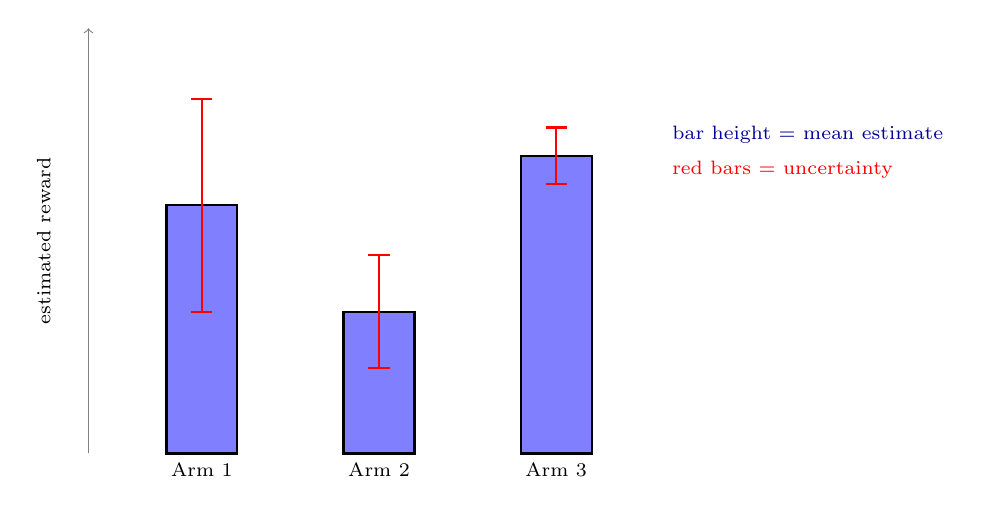
\begin{tikzpicture}[scale=0.9]
  % Three arms, each with mean estimate and confidence interval
  \foreach \i/\mean/\ci/\label in {1/3.5/1.5/Arm 1, 2/2.0/0.8/Arm 2, 3/4.2/0.4/Arm 3} {
    \fill[blue!50] (\i*2.5 - 1.5, 0) rectangle (\i*2.5 - 0.5, \mean);
    \draw[thick] (\i*2.5 - 1.5, 0) rectangle (\i*2.5 - 0.5, \mean);
    \draw[thick, red] (\i*2.5 - 1.0, \mean - \ci) -- (\i*2.5 - 1.0, \mean + \ci);
    \draw[thick, red] (\i*2.5 - 1.15, \mean - \ci) -- (\i*2.5 - 0.85, \mean - \ci);
    \draw[thick, red] (\i*2.5 - 1.15, \mean + \ci) -- (\i*2.5 - 0.85, \mean + \ci);
    \node[font=\scriptsize, anchor=north] at (\i*2.5 - 1.0, 0) {\label};
  }
  \draw[->, gray] (-0.1, 0) -- (-0.1, 6);
  \node[font=\scriptsize, rotate=90, anchor=south] at (-0.5, 3) {estimated reward};
  \node[font=\scriptsize, anchor=west] at (8, 4.5) {\textcolor{blue!60!black}{bar height = mean estimate}};
  \node[font=\scriptsize, anchor=west] at (8, 4) {\textcolor{red}{red bars = uncertainty}};
\end{tikzpicture}
\caption{A three-armed bandit after some number of pulls. Arm 1 has been pulled some; the estimate is decent but the uncertainty is large. Arm 2 has been pulled a fair amount and looks worse than Arm 1. Arm 3 has the highest estimate and the tightest uncertainty. The pure exploiter plays Arm 3 always. The pure explorer keeps pulling all three. A good policy plays Arm 3 most of the time but occasionally pulls Arm 1 (whose true mean might be above its estimate, given the large uncertainty).}
\label{fig:bandit}
\end{figure}

Several practical policies balance exploration and exploitation.

\textbf{Epsilon-greedy.} With probability $1 - \epsilon$, take the best-known action. With probability $\epsilon$, take a random one. Simple, widely used, has known suboptimalities.

\textbf{UCB (upper confidence bound).} At each step, pick the action that maximizes ``best estimate plus uncertainty.'' Concretely: choose the arm maximizing $\hat{\mu}_a + c\sqrt{\log t / n_a}$, where $\hat{\mu}_a$ is the empirical mean, $n_a$ is the number of pulls so far, and $c$ is a constant. The agent is optimistic about arms it has not tried much, because their uncertainty term is large. Auer, Cesa-Bianchi, and Fischer (2002).

\textbf{Thompson sampling.} Maintain a probability distribution (a posterior) over each arm's parameter. At each step, sample once from each posterior; play the arm whose sample is highest. Bayesian, often near-optimal, has clean theoretical guarantees.

What all three have in common: they treat ``how much I do not know'' as itself a quantity to factor into decisions. Uncertainty is not just a problem; it is a signal.

\section*{The value of information}

How much is knowing worth?

Howard (1966) gave the mathematical answer. The \emph{value of information} of an observation $o$ is the expected improvement in decision quality from receiving it:

$$\mathrm{VoI}(o) = \mathbb{E}\big[\max_a EU_{\text{after }o}(a)\big] - \max_a EU_{\text{before}}(a).$$

The first term is the expected value of acting optimally after observing $o$, averaged over what $o$ might turn out to be. The second is the expected value of acting optimally without the observation. The difference is what the observation is worth.

VoI is what exploration-exploitation policies are computing, in disguise. Each policy is a rule of thumb that approximates ``would the information gained from trying this action be worth more than the reward I would forgo by not exploiting?''

The general lesson: information has a price. Optimal agents do not just maximize current expected utility. They also weigh how much each action would teach them, because tomorrow's decisions can be better if today's action provides useful data.

\section*{Where this leaves you}

You now have the engineering picture of optimal agency. The agent operates in a state-action-reward loop. Its goal is to maximize discounted reward. Its knowledge is encoded in value functions or Q-functions. It learns by experience using algorithms like Q-learning. It balances exploration and exploitation using the value of information, implicit in policies like UCB and Thompson sampling.

Two issues are unresolved.

The first is engineering. Tabular Q-learning works on toy problems but does not scale. Chess has about $10^{44}$ legal positions; Go has about $10^{170}$; even Pac-Man has more states than an agent can visit. Almost every real state is new. A tabular agent cannot say anything about a state it has not seen. To handle real problems, the agent has to generalize from the states it has seen to ones it has not.

The second is theoretical. We have an optimal predictor (Solomonoff, Part I) and an optimal decider (expected utility maximization, Chs 5-6). They are not yet combined.

\textbf{Chapter 7 (Generalization)} takes up the first issue. Function approximation replaces the table; learned representations let the agent extrapolate; inductive biases are what make the extrapolation work; Solomonoff appears at the limit. This is the conceptual bridge between optimal-agent theory and practical-agent reality.

\textbf{Chapter 8 (AIXI)} takes up the second. Solomonoff induction for the belief; expected utility maximization for the action; together, AIXI. The optimal universal agent. Uncomputable, but the right reference point.

\textbf{Chapter 9 and beyond (Part III)} return to the question Chapter 5 deferred: where does the utility function come from? Specifying it is the hardest part of building intelligent agents. Goodhart's law is the structural warning. The alignment problem is what follows when the specification fails at scale. That problem gets its own part.

The next chapter takes up generalization.
